\documentclass[../manifest.tex]{subfiles}

% - should include scenarios of use and multiple screenshots of your software in action. walk the reader through how your interface succeeds (or acknowledge how it falls short) in solving the intended problem.
% - if you did any evaluation (deployment to target users, computational benchmarks), do report on that here.

\begin{document}

Teamline was designed specifically for the use-case of supporting TAs in grading students for the course \textit{CPSC 310 Introduction to Software Engineering} at the University of British Columbia\footnote{See section TODO for elaboration on how the domain can be extended.}. The course is characterized by multiple deliverables and a retrospective session after each deliverable with the TA and each team member individually. Currently, students are required to hand in an individual contribution file for each deliverable that points out how they contributed to their implementation, outlining their major commits and evaluating what went well or bad during the 'sprint'. Figure~\ref{fig:sample-contribution-file} shows an example contribution file.

\begin{figure}[h]
  \centering
  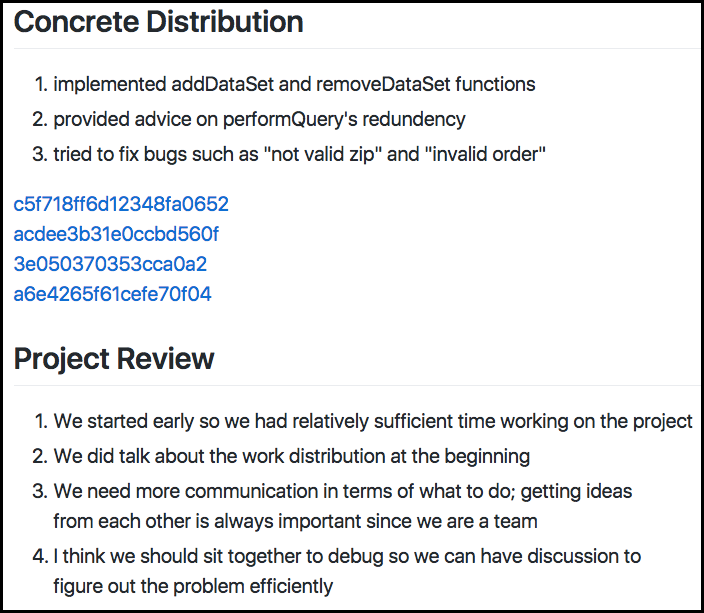
\includegraphics[width=\linewidth]{sample-contribution-file}
  \caption{Sample contribution file}
  \label{fig:sample-contribution-file}
\end{figure}

Using this contribution file as a basis, the TA will then talk to the team members and try to assess if they contributed evenly to the deliverable. The TA may use information provided by Github, like the deliverable's commit history and contribution graphs (see Figure~\ref{fig:sample-contribution-graph}) to obtain a better picture for the assessment. If an uneven contribution is visible, the TA is then to downscale the team member who contributed less gradually. As described earlier, this assessment can be a very challenging task with only the information provided.

\begin{figure}[h]
  \centering
  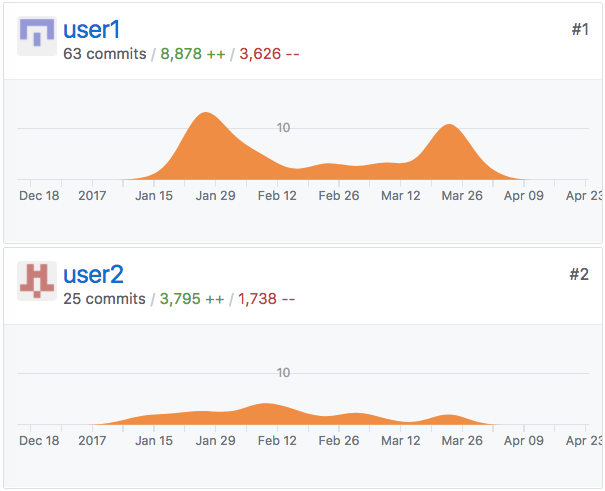
\includegraphics[width=\linewidth]{sample-contribution-graph}
  \caption{Sample contribution graph showing number of commits and code churn by contributor}
  \label{fig:sample-contribution-graph}
\end{figure}

Teamline makes this assessment significantly easier. In this sample scenario, the TA is to assess the contribution of each member in \textit{Team127}, from which the previous sample contribution file and graph (figures~\ref{fig:sample-contribution-file} and~\ref{fig:sample-contribution-graph}) were taken. In the overview, the TA is given a first picture of the team's final grade and distribution of contribution (see figure~\ref{fig:sample-overview} with Team127 highlighted). Although the contribution file from \textit{User1} (figure~\ref{fig:sample-contribution-file}) would indicate that contribution to the deliverable was distributed fairly and both team members tell the TA exactly that, the TA will see immediately that the team cell has a dark orange color (highly saturated color indicating uneven distribution) and become suspicious upon the students' statements.

The TA then clicks on the table cell and the team view appears (see figure~\ref{fig:sample-teamview}). The left chart shows the team's general performance with a very good final grade (blue line) of 99\%. Both pass rate (orange line) and coverage (green line) switched significantly back and forth during progress on the deliverable which often indicates regression bugs in the team's code and out- and uncommenting parts of their code. More significant than the overall performance is the unequal distribution of contribution visible in the two contribution charts on the right. Whereas the chart for User2 on the right shows almost linear improvements in pass rate (blue line) and coverage (green line), both lines remain at 0\% on the y-axis for User1 on the left side. This indicates that -- by bare numbers -- User1 was not responsible for any improvements on pass rate and coverage in this deliverable and contribution was highly uneven. The charts also tell that User1 is the author of only 4 commits while User2 is responsible for 16 commits, which is another indicator for uneven contribution.

In this scenario, the TA therefore has a much better picture of how each team member contributed and will very likely downscale User1 and/or give more credits to User2.

\end{document}
